\newpage
\subsection{Working with multiple EAPs}
\visHeader
\label{sec:multiEAP}

\begin{itemize}

\item[$\blacktriangleright$] Included in the \texttt{Part4} .zip file is \texttt{dictionaryLanguage.eap}. Double click this to open it in
Enterprise Architect (EA).

\vspace{0.5cm}

\item[$\blacktriangleright$] Although you can simply copy and paste single packages between multiple EAPs, packages with dependencies to other packages (i.e.,
those between \texttt{DictionaryCodeAdapter} and \texttt{DictionaryLanguage}) cannot be copied so easily. If you do this, all links will be destroyed!
Therefore, to migrate multiple packages, you have to first export a \emph{complete} root node (the package on the top-most level of the project browser) to an
XMI file.

\vspace{0.5cm}

\item[$\blacktriangleright$] Right click on \texttt{dictionaryLanguageRoot}, and select \texttt{Export Model to XMI\ldots,} as depicted in
Fig.~\ref{fig:export}.

\vspace{0.5cm}

\begin{figure}[htbp]
\begin{center}
  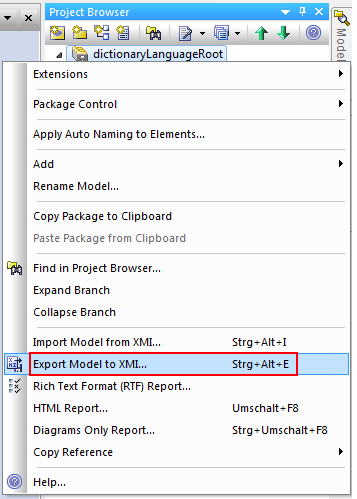
\includegraphics[width=0.5\textwidth]{ea_exportToXMI}
  \caption{Exporting the \emph{target metamodel}}
  \label{fig:export}
\end{center}
\end{figure}

\item[$\blacktriangleright$] Save the file somewhere easily accessible, such as your desktop, and change the export type to \texttt{XMI 2.1}. You should have a
small green bar appear once the action is complete (Fig.~\ref{fig:exportDialogue}).

\vspace{0.5cm}

\begin{figure}[htbp]
\begin{center}
  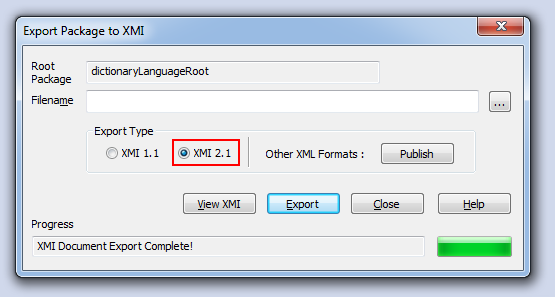
\includegraphics[width=0.8\textwidth]{ea_exportPackageDialogue}
  \caption{Persisting the export to a file}
  \label{fig:exportDialogue}
\end{center}
\end{figure}

\item[$\blacktriangleright$] Now open your \texttt{LeitnersLearningBox.eap} file, and right-click the root \texttt{MyWorkingSet} node and select \texttt{Import
Model from XMI\ldots}. In the dialogue that appears, find the file you just saved and \texttt{import}. Press \texttt{yes} in each of the confirmation dialogues
that appear after. Your workspace should now resemble Fig.~\ref{fig:postImport}.

\vspace{0.5cm}

\begin{figure}[htbp]
\begin{center}
  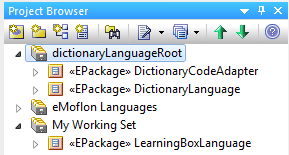
\includegraphics[width=0.5\textwidth]{ea_postImport}
  \caption{Project explorer after importing the \emph{target} metamodel}
  \label{fig:postImport}
\end{center}
\end{figure}

\end{itemize}
